\chapter{Wykorzystane technologie}

\section{Xcode i Developer Tools}
Xcode jest IDE (Integrated development environment) stworzonym przez Apple i dostępnym za darmo do pobrania z App Store, sklepu z aplikacjami do którego dostęp mają wyłącznie użytkownicy komputerów z systemem MacOS. Jest wyposażony w pakiet wszystkich narzędzi (Developer Tools) potrzebnych dla developerów aby tworzyć aplikacje na iOS. Główną aplikacją pakietu jest Xcode IDE który wraz z wspomagającymi aplikacjami dostępnymi w pakiecie takimi jak Simulator czy Instruments czyni pracę przy tworzeniu aplikacji płynną i efektowną. W tym rozdziale przedstawię właśnie te narzędzia ze względu na ich rolę w procesie tworzenia aplikacji.

\begin{figure}[ht!]
  \centering
  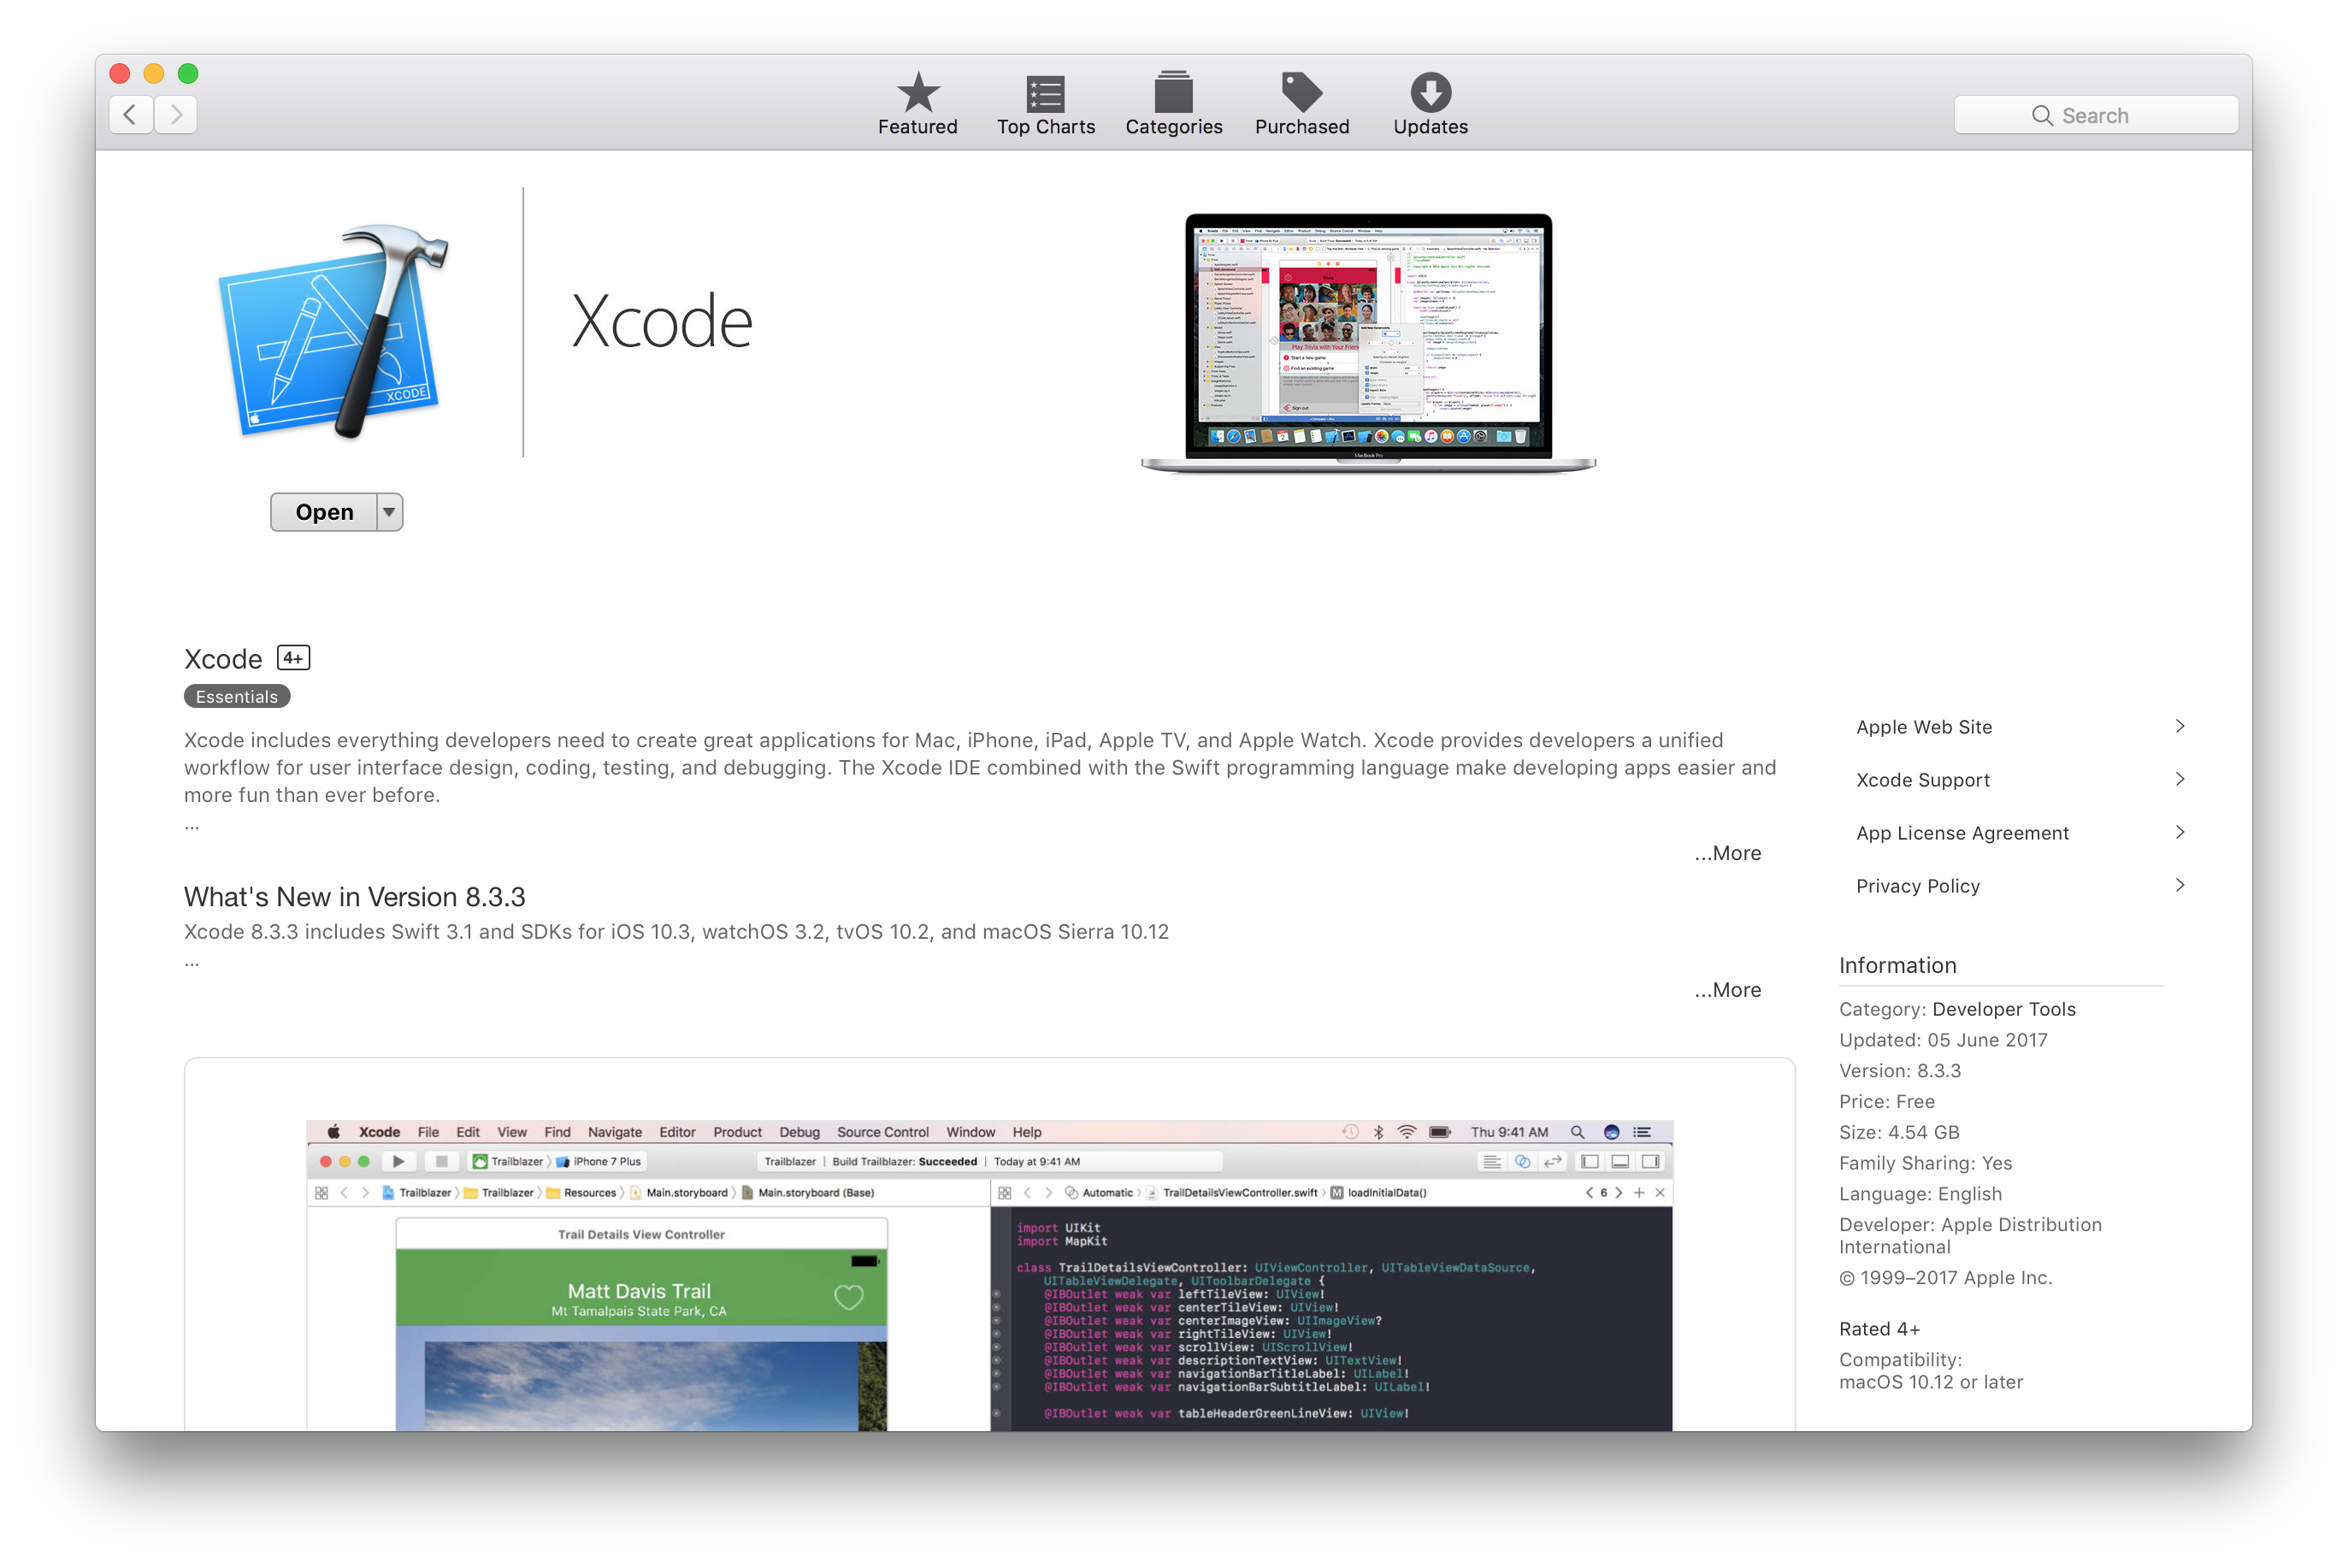
\includegraphics[width=120mm]{images/chapter-2-image-1-appstore.png}
  \caption{Xcode w App Store}
  \label{chapter-2-image-1-appstore}
\end{figure}

\subsection{Xcode IDE}
Xcode jako nowoczesne, produktywne środowisko jest miejscem w którym programista aplikacji na iOS spędza większość swojego czasu. Całość prac wykonywanych przy produkcji aplikacji może zostać wykonana właśnie tutaj. Najbardziej podstawowy element jakim jest edytor tekstu dobrze współgra z takimi narzędziami jak Interface Buildier, który pozwala w prosty sposób zaprojektować stronę wizualną aplikacji przy użyciu Storyboardów a następnię stworzyć referencję w kodzie do wybranych przez nas elementów przez proste przeciągnięcie myszką. Storyboardy są opcjonalnym aczkolwiek bardzo pożytecznym narzędziem szczególnie dla programistów stawiających swoje pierwsze kroki na tej platformie. Zapewniają one wizualne wyobrazenie interfejsu aplikacji nad którą wykonywana jest praca, a projektowanie dowolnego widoku który będzie wyglądał dobrze na każdym urządzeniu w dowolnej orientacji, jest relatywnie proste po zapoznaniu się z kilkoma elementarnymi zasadami.

\begin{figure}[ht!]
  \centering
  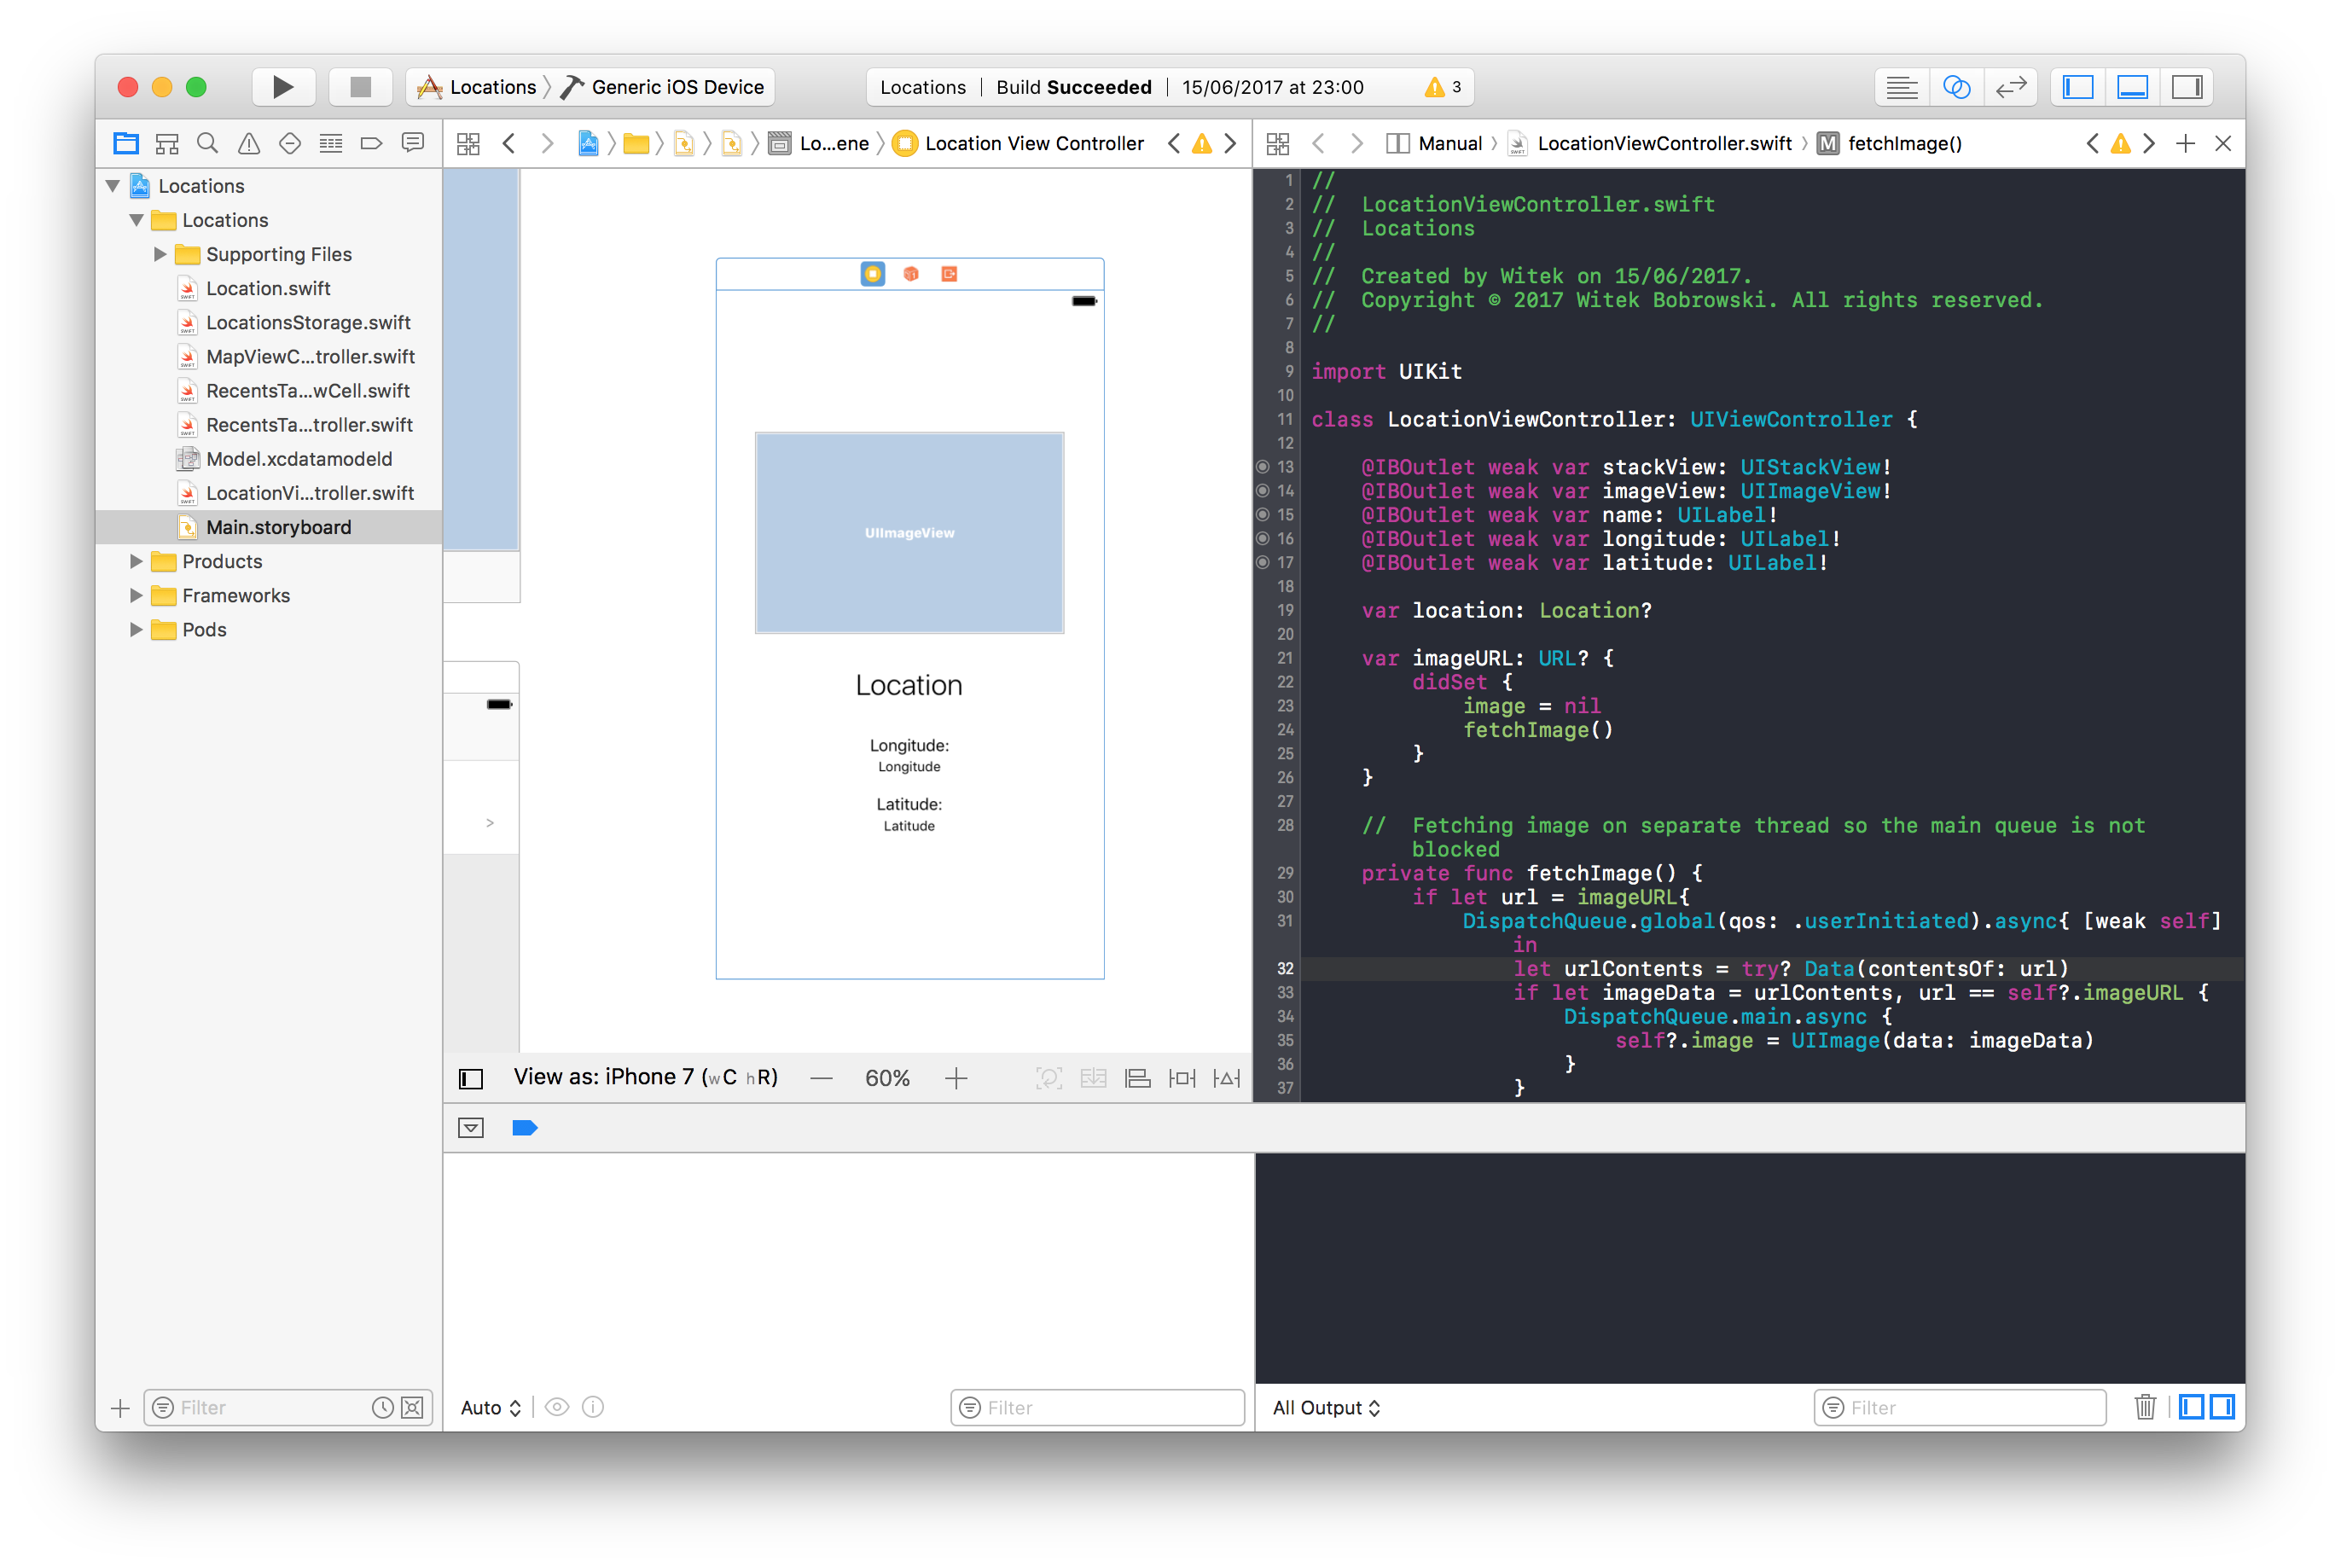
\includegraphics[width=120mm]{images/chapter-2-image-2-xcode.png}
  \caption{Xcode pokazujący "Assistant editor"}
  \label{chapter-2-image-2-xcode}
\end{figure}

Ponieważ Storyboardy tworzy się w jednym pliku o formacie .storyboard, często w profesjonalnej produkcji rezygnuje się z nich ze względu na konflikty w systemach kontrolii wersji. Konflikty te powstają w wyniku pracy wielu programistów, a ponieważ plik .storyboard jest w rzeczywistości plikiem XML, który został wygenerowany automatycznie, rozwiązywanie konfilków bywa kłopotliwe, a przy dużych projektach problematyczne. Dlatego rezygnuje się z nich na rzecz tworzenia widoków tylko przy użyciu kodu, oraz niezależnych plików XIB. Pliki te pozwalają na ustawienie elementów w stylu znanym ze Storyboardów lecz w przeciwieństwie do nich reprezentrują pojedyńczy widok, dzięki czemu problem z konfliktami zostaje uniknięty a jednocześnie tworzenie bardziej skomplikowanych widoków pozostaje znacznie ułatwione. Xcode zapewnia wsparcie dla systemu kontroli wersji git. Przy tworzeniu nowego projektu, gdy jest o to poproszony, inicjalizuje nowe repozytorium. Dodatkowo w nawigatorze projektu, w którym widać strukturę projektu, Xcode oznaczy literą "M" pliki które git oznacza jako pliki w których dokonano zmian (modified) a literą "A" pliki które zostały dodane (new file) od czasu poprzedniego zachowania zmian.
W najnowszej wersji 9.0, Xcode zyskał nową funkcjonalność - Source Control Navigator, który pozwala na eksplorowanie poszczególnych gałęzi repozytorium i podglądu dowolnego momentu w jego historii.

\subsection{Simulator}
Simulator pozwala na uruchomienie zbudowanej aplikacji na dowolnym urządzeniu z iOS które jest w stanie zasymulować. Gdy chce się przetestować aplikację wystarczy w pasku narzędzi Xcode wybrać dowolny model urządzenia (oprócz telefonów iPhone znajdują się tam rówież tablety iPad) które chcemy zasymulować (jeżeli podłączymy do komputera fizyczne urządzenie, Xcode rówiez je wykryje i pozwoli na zainstalowanie i uruchomienie na nim aplikacji), a Xcode przejdzie to etapu budowania aplikacji w którym kompiluje pliki źródłowe, a następnie umieści aplikację w symulatorze wybranego przez nas urządzenia.

\begin{figure}[ht!]
\centering
\begin{subfigure}{.5\textwidth}
  \centering
  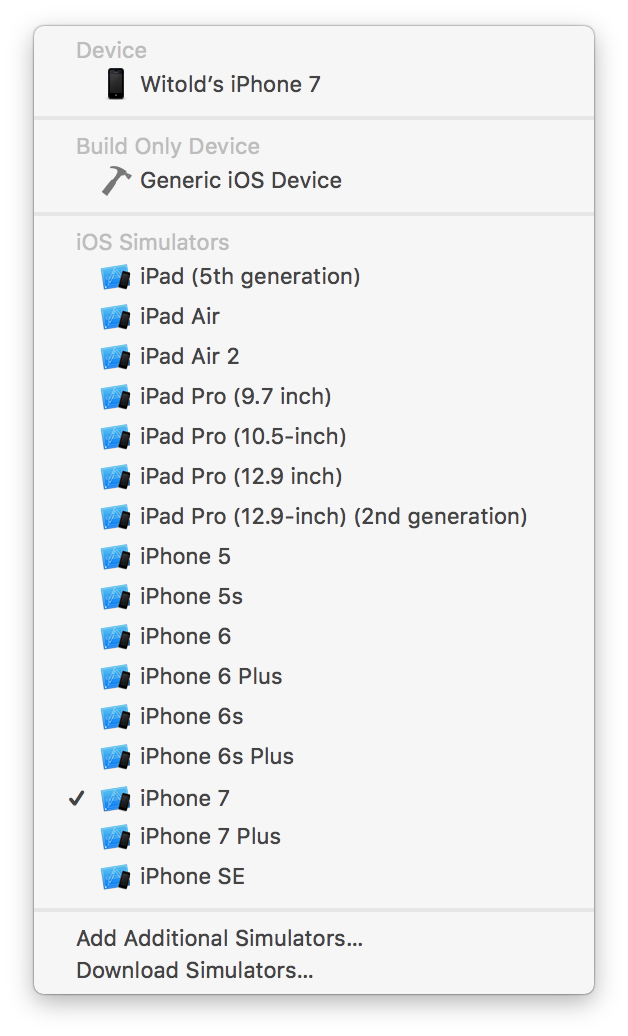
\includegraphics[width=.4\linewidth]{images/chapter-2-image-3-target.png}
  \caption{Wybór docelowego urządzenia}
  \label{chapter-2-image-3-target}
\end{subfigure}%
\begin{subfigure}{.5\textwidth}
  \centering
  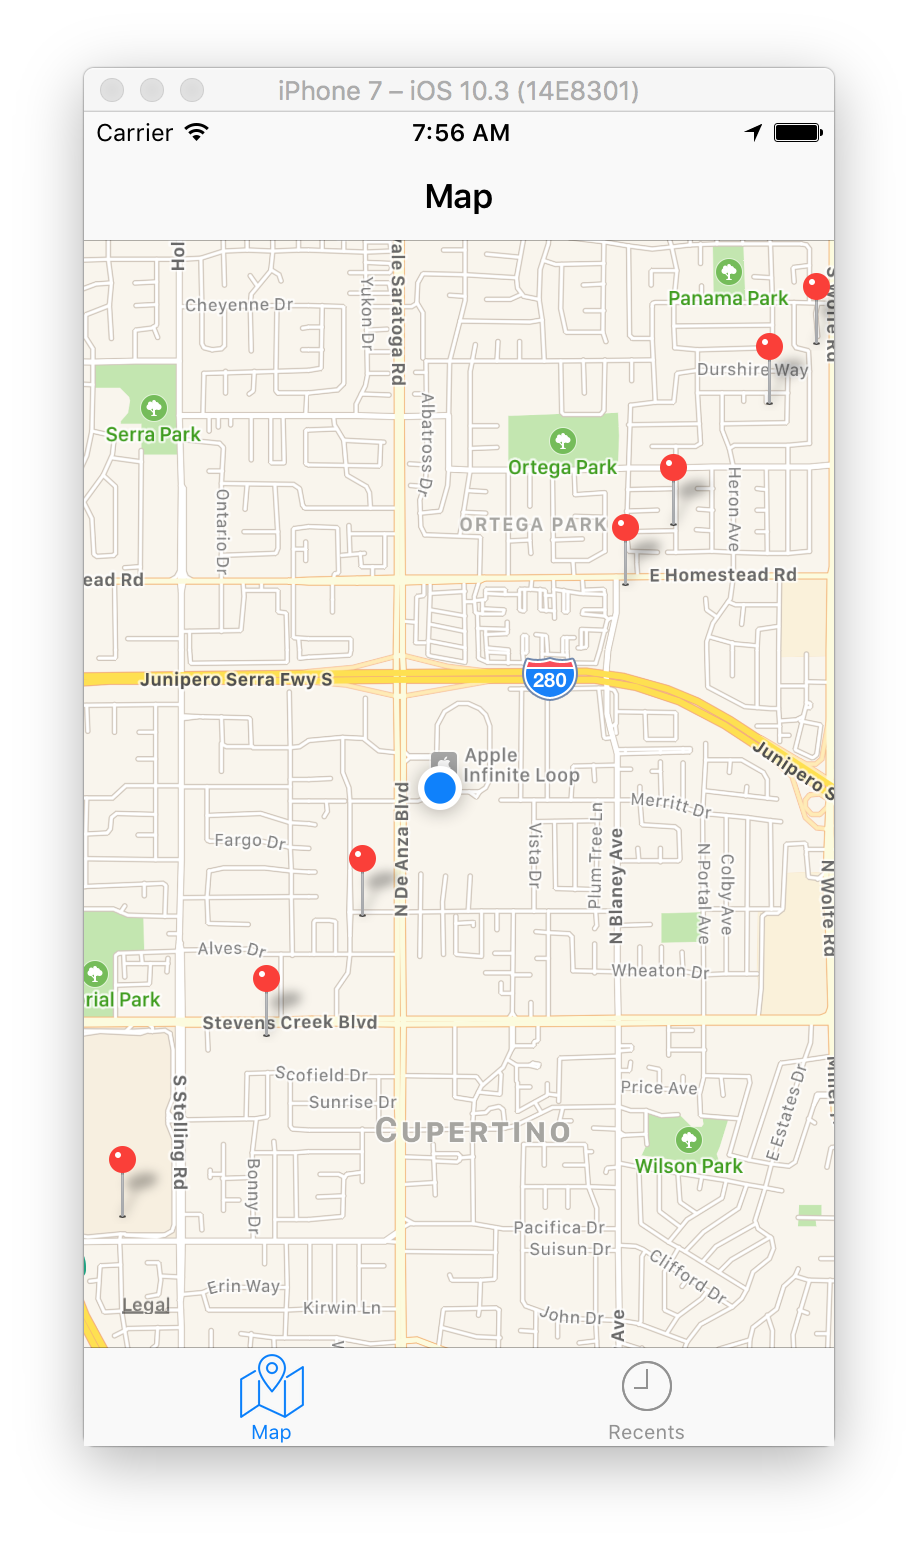
\includegraphics[width=.4\linewidth]{images/chapter-2-image-4-simulator.png}
  \caption{Uruchomiona aplikacja na iPhone 7}
  \label{chapter-2-image-4-simulator}
\end{subfigure}
\caption{Po wybraniu urządzenia w Xcode, Simulator uruchamia na nim aplikację}
\label{chapter-2-image-4-5}
\end{figure}

Podczas gdy aplikacja jest uruchomiona i testowana na symulatorze, Xcode pozwala na podgląd użycia zasobów takich jak procesor, pamięć RAM, pamięć dyskowa oraz sieć. Po wybraniu dowolnego z wyżej wymienionych zasobów z nawigatora Debuggera ukazje nam się bardziej szczegółowy podgląd na to w jakim stopniu aplikacja obciąża urządzenie co pozwala na szczegółowe testowanie.

\begin{figure}[ht!]
  \centering
  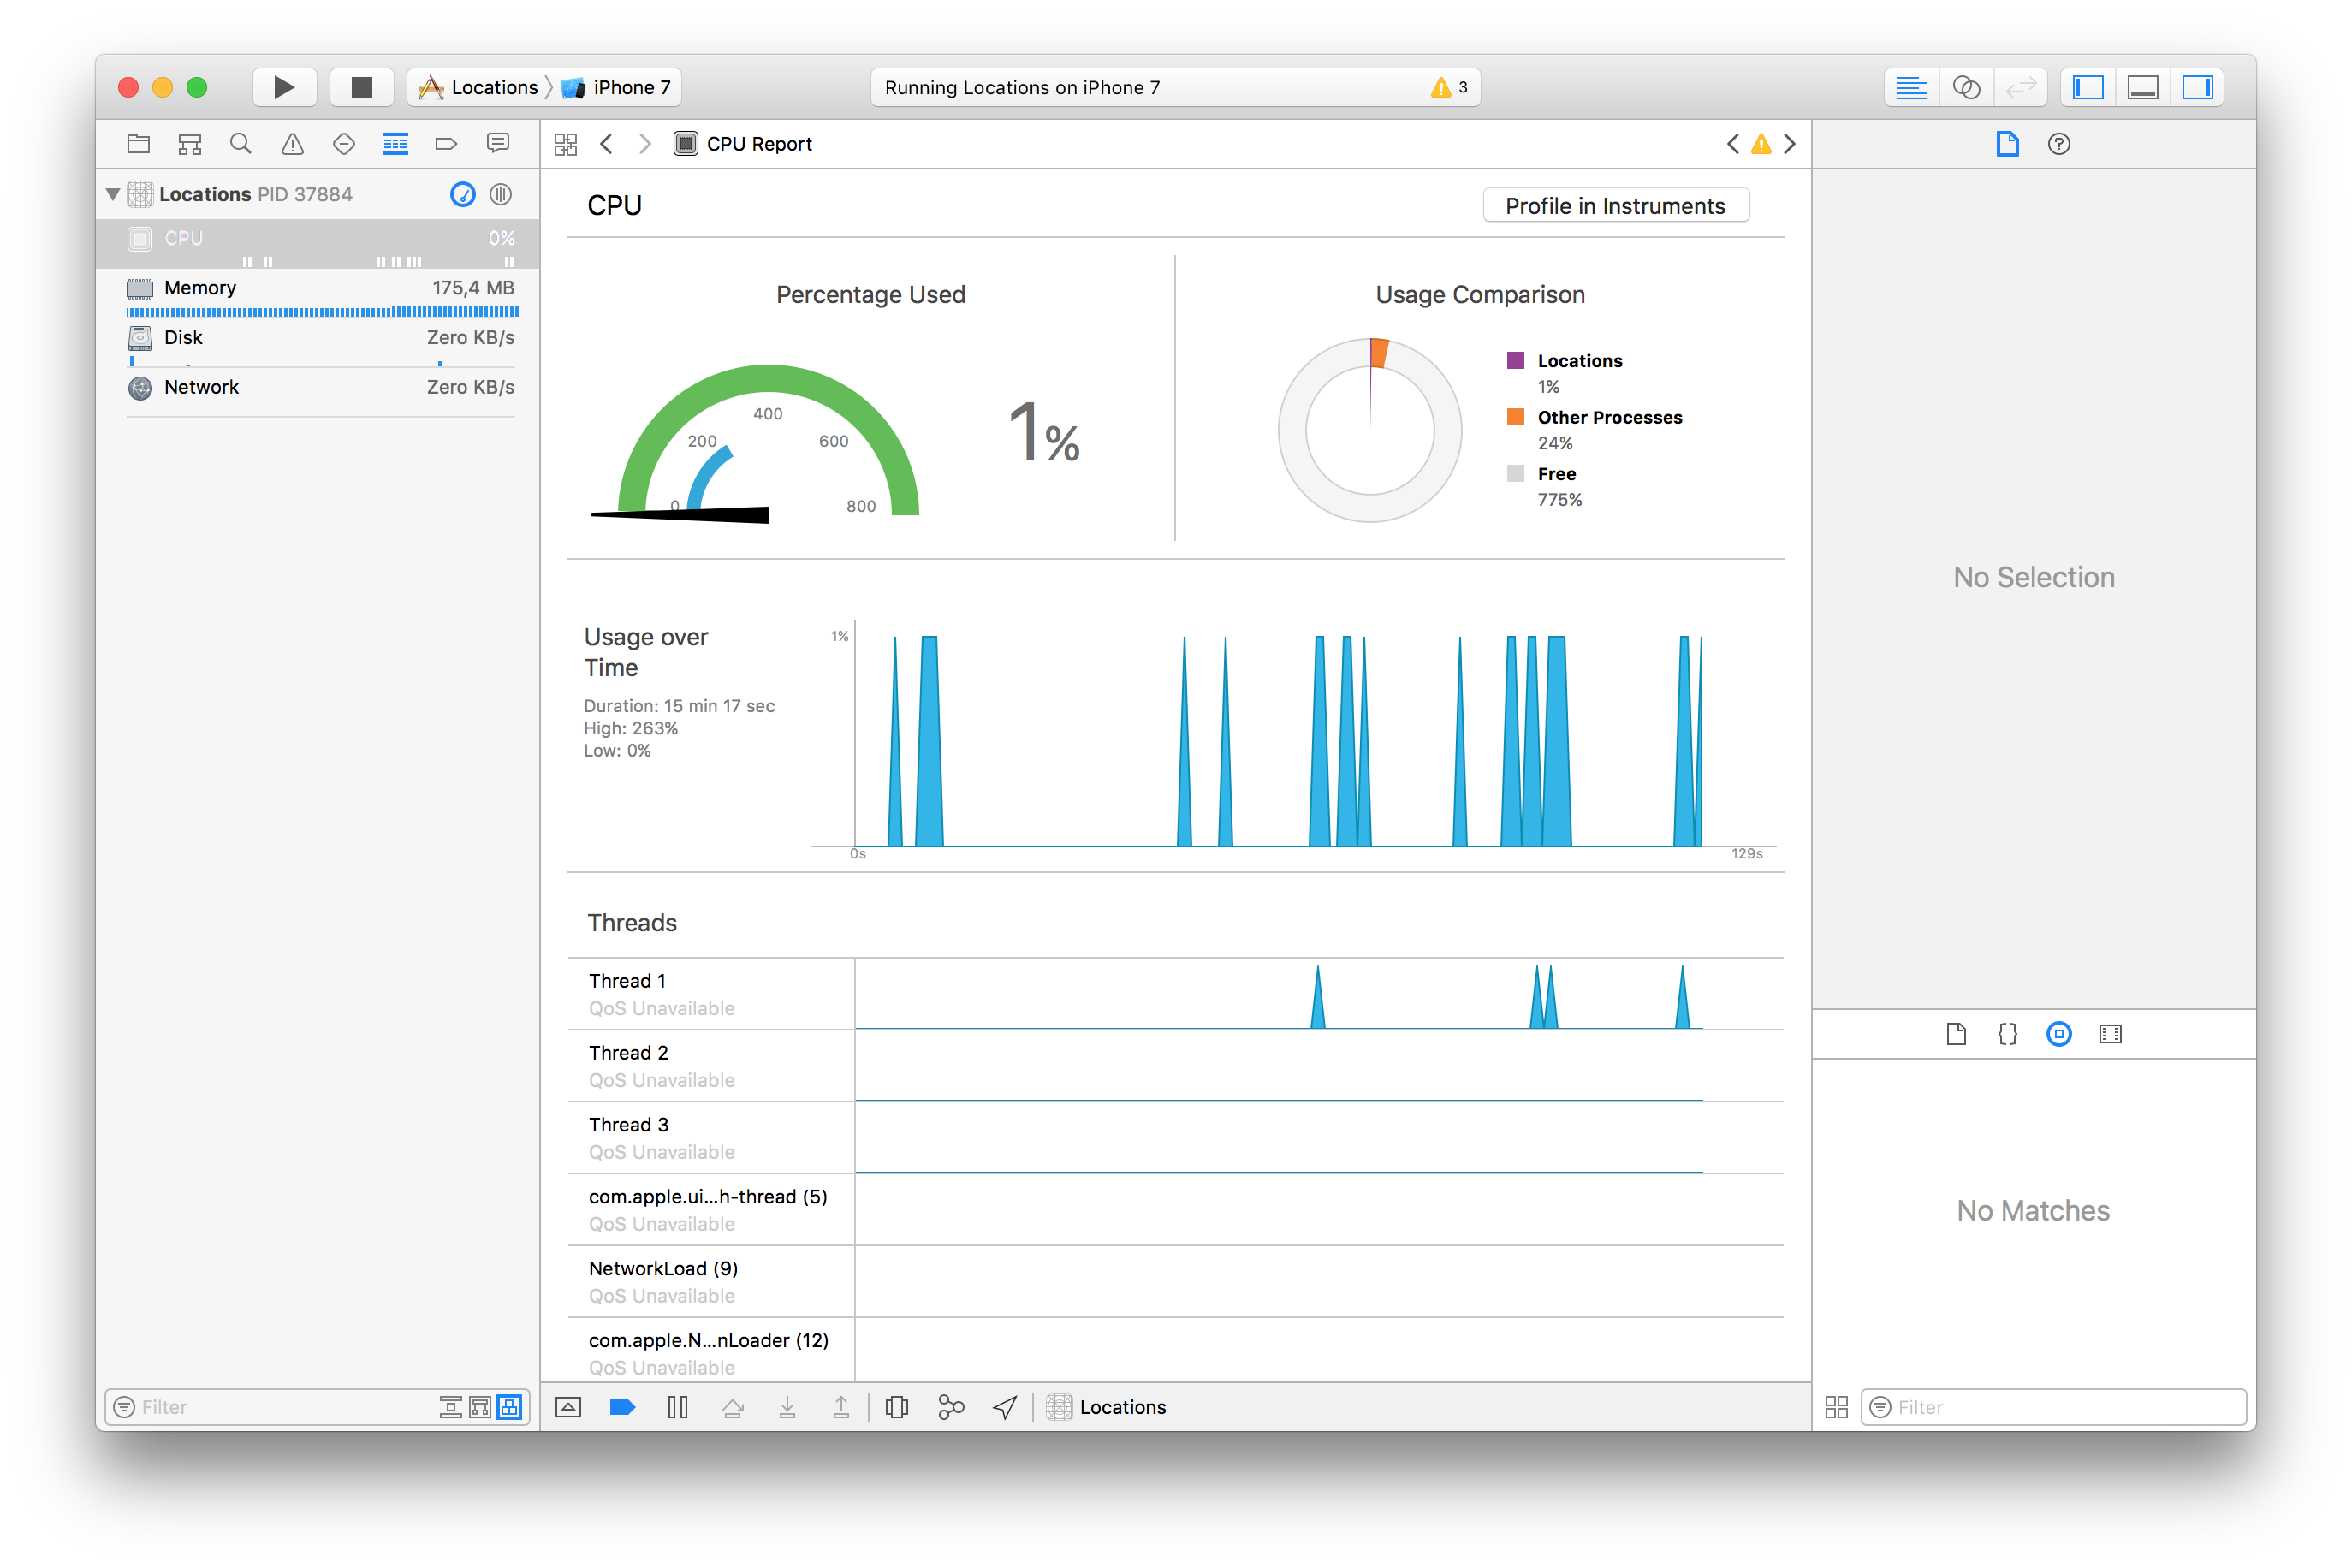
\includegraphics[width=120mm]{images/chapter-2-image-5-debugger.png}
  \caption{Użycie CPU na symulatorze odświeżane na bieżąco i wyświetlne w Xcode}
  \label{chapter-2-image-5-debugger}
\end{figure}

\subsection{Instruments}

Widok poboru zasobów w Xcode jest bardzo pomocny na poglądową ocenę wydajności naszej aplikacji, jeżeli jednak chcemy poddać ją prawdziwej próbie, musimy uruchomić kolejne narzędzie jakim jest Instruments. Instruments jest aplikacją dzięki której dokonamy pomiaru nie tylko każdego zasobu na urządzeniu, ale również dostajemy możliwość nadzoru takich aktywności jak alokowanie pamięci dla obiektów, zmiany layoutu widoków czy zmiany w Core Data, natywnej bazie danych dla iOS.

\begin{figure}[ht!]
  \centering
  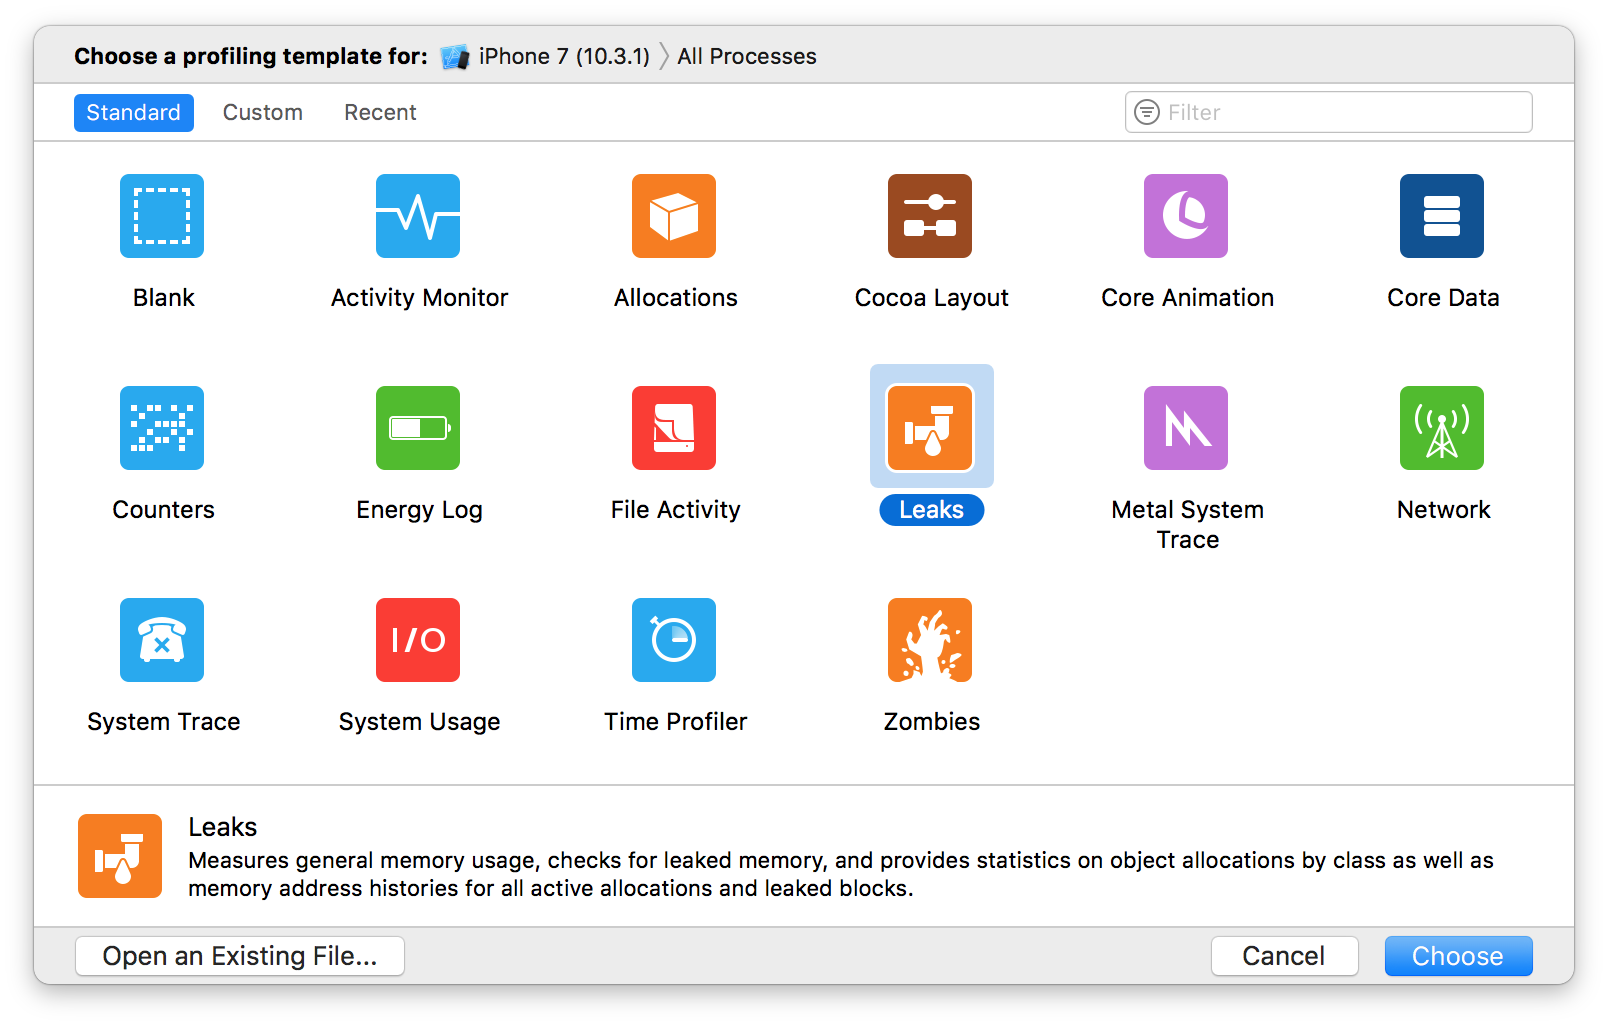
\includegraphics[width=120mm]{images/chapter-2-image-6-instruments.png}
  \caption{Instruments, menu główne}
  \label{chapter-2-image-6-instruments}
\end{figure}

Niezależnie od tego jak szybkie i wydajne są w dzisiejszych czasach telefony, optymalny kod nadal jest podstawą prawidłowego działania aplikacji i niedbałe projektowanie architektury może być fatalne w skutkach. Cykle referencji mogą powodować niechciane wycieki pamięci a problemy powstające podczas przerysowywania się widoków spowodują nieczytelny interfejs. Jeżeli takie błędy nie zostaną wykryte na etapie produkcyjnym, a dogłębne testy aplikacji nie zostaną przeprowadzone przed oddaniem jej do recenzji (Aby nasza aplikacja mogła znależć się w sklepie AppStore, i być dostępna dla każdego, musi ona otrzymać pozytywną recenzje Apple) aplikacja najprawdopodobniej zostanie odrzucona, co wiąże się z dodatkowymi opóźnieniami. Pakiet narzędzi dostarczanych przez Apple spełnia swoje zadanie i dla większości developerów są one wystarczające. Istnieją rozwiązania firm trzecich, JetBrains dostarcza alternatywne IDE do produkcji aplikacji - AppCode, które cieszy się bardzo dobrą reputacją wśród użytkowników.

\section{Swift}

\subsubsection*{Hello, world!}

Gdy w 1996 roku Apple przejęło NeXT wraz z ich oprogramowaniem, Objective-C stało się głównym językiem do tworzenia oprogramowania na najnowszy system operacyjny OS X. Wraz z OpenStepem Apple znalazło się w posiadaniu takich narzędzi jak Interface Buildier oraz Project Buildier które z biegiem czasu ewoluowały w Xcode który znamy dzisiaj. Objective-C służył programistom przez wiele lat, na początku tym tworzącym aplikacje desktopowe, a od ukazania się pierwszego iPhone'a, programistom mobilnym. Objective-C jest bardzo mocno rozwiniętym językiem, co zwarzając na jego wiek niepowinno nikogo dziwić. Lecz jako język którego początki sięgają wczesnym latom osiemdziesiątym dwudziestego wieku, z biegiem lat postarzał się, co bardzo upraszczając można by przedstawić stwierdzeniem, iż nie jest wystarczająco nowoczesny.

Twórca LLVM (Low Level Virtual Machine) Chris Lattner, w 2010 roku rozpoczął prace nad nowym językiem który z założenia miał czerpać inspirację z takich języków jak Objective-C, Haskell, Python czy Ruby. Cztery lata później, Apple na WWDC (Worldwide Developer Conference) zaprezentowało Swifta i wypuściło wersję beta. Swift jest bezpiecznym, szybkim językiem, który agreguje wiele paradygmatów znanych z innych nowoczesnych języków. Jego najważniejszymi cechami są automatycznie zarządzana pamięć, typ Opcjonalny który zapewnia wsparcie dla nullowych wskaźników, zaawansowana obługa błędów która zapewnia kontolowane wyjście z niespodziewanych niepowodzeń, zmienne, które zawsze są zainicjalizowane przed użyciem oraz silne typowanie które po połączeniu z nowoczesnym, lekkim syntaxem czyni go językiem zarówno potężnym jak i łatwo dostępnym. Dynamiczny rozwój zawdzięcza inżynierom z Apple oraz społeczności open-source, którzy bardzo intensywnie pracują dodając nowe elementy, naprawiając niedoskonałości oraz optymalizując jego architekturę. Swift dzisiaj jest jednym z najbardziej lubianych języków programowania. Jego popularność wciąż rośnie, a odkąd stał się projektem open-source'owym oprócz systemów Apple, zaczyna być uzywany do takich celów jak tworzenie serwerowych aplikacji. Zdominował platformę iOS i zdetronizował Objective-C, stając się jezykiem pierwszego wyboru. Wszystkie powstające aplikacje są tworzone przy jego użyciu, i wiele napisanych w Objective-C jest dzisiaj przepisywanych na nowy język. Warto wspomnieć, że kod w Objective-C i kod w Swifcie może być użyty w tej samej aplikacji, dzięki czemu może się tam znaleźć równieź C i C++. Jednak aby użyc kodu napisanego w C czy w C++ w Swifcie musimy go najpierw opakować aby był dla niego dostępny. W przypadku Objective-C, Swift ma dostęp do jego obiektów oraz może dziedziczyć z jego klas. A to zapewnia nam dostęp do wszystkich natywnych bibliotek, czyniąć Swift pełnoprawnym językiem i narzędziem gotowym do użytku już w dniu jego premiery.

Do projektu wykorzystano Swift w wersji 3.1.

\section{iOS SDK}

Jak już wspomniano wcześniej, iOS dziedziczy wiele po desktopowym systemie, MacOS. W skład iOS SDK wchodzą biblioteki znane już od wielu lat oraz biblioteki stworzone z myślą o urządzeniach mobilnych. W tej sekcji omówiono po krótce framework CocoaTouch, który dostarcza elementy interfejsu będące podstawą każdej aplikacji i zapewniajce wizualną spójność platformy.

\subsection{CocoaTouch}

CocoaTouch jest potomkiem frameworku Cocoa dostępnego na systemach MacOS który jest rozszeżony o interfejs obsługi narzędzi dostępnych w urządzeniu mobilnym takich jak rozpoznawanie gestów, serwis lokalizacji czy obsługa kamery. W skład CocoaTouch wchodzą między innymi biblioteki Foundation, UIKit, MapKit, EventKit i wiele innych. Dzięki temu pakietowi Apple zdefiniowało jak powinny byc tworzone aplikacje na iOS. Dostarczony jest zbiór wielu elementów interfejsu uzytkownika które można dowolnie rozszeżać i modyfikować aby stworzyć unikalny wygląd aplikacji trzymając się wytycznych wyznaczonych przez Apple. Dostęp do gestów zapewni naszej aplikacji lekkość obsługi oraz intuicyjność, a niezliczona ilość innych biblitotek wchodzących w skład CocoaTouch sprawi że aplikacja nabierze życia. Implementowanie funkcjonalności staje się bardzo proste dzięki wysoko poziomowym interfejsom dającym dostęp do poszczególnych elementów systemu oraz fizycznego urządzenia. CocoaTouch jest najbardziej elementarnym frameworkiem na iOS ponieważ to on zapewnia na poziomie postawowym to co potrzebne do stworzenia funkcjonalnej aplikacji. Zakładając że aplikacja powinna agregować, w jakiś sposób przetwarzać a następnie wyświetlić w odpowiedniej formie zbiór pewnych danych, CocoaTouch w parze ze Swiftem to zagwarantują, oczywiście do pewnego stopnia. W większości przypadków gdy potrzebujemy wykonać jakieś specyficzne zadanie, lub chcemy je poprostu uprościć unikając implementacji własnego rozwiązania problemu co było by czasochłonne, będziemy skłaniać się ku zewnętrznym bilbiotekom.

\section{Zewnętrzne biblioteki}

Biblioteki te, tworzone przez środowiska open-sourcowe, pojedyńczych programistów czy wielkie korporacje dadzą nam to czego nie otrzymaliśmy wraz z natywnymi frameworkami. Przykładem jest projekt który opisuje ta praca. Rozwiazuje problem programisty tworzącego własną aplikację króry nie chce tracić czasu na implementowanie funkcjonalości która zajęła by mu relatywnie dużo czasu, a która niekoniecznie jest głównym celem jego aplikacji. Istnieje wiele sposobów na rozszeżenie naszej aplikacji o wybrane moduły, które bardziej szczegółowo zostaną opisane pod koniec czwartego rozdziału podczas omawiania możliwościach dystrybucji framewoku. W tej sekcji przedstawiono framework'i wykorzystane do projektu EPUKit, które nie wchodzą w skład iOS SDK a zostały udostępnione do publicznego użytku.

\subsection{Zip}

Zip jest swift'ową biblioteką open-source dostępną na licencji MIT której kod źródłowy znajdziemy na GitHubie\footnote{Adres url: \href{https://github.com/marmelroy/Zip}{github.com/marmelroy/Zip}}. Zip jest narzędziem do archiwizowania plików oraz rozpakowywania archiwów. Wspiera on formaty archiwów .zip, .cbz oraz daje możliwość dodania rozszeżenia pliku który chcemy rozpakować. W przypadku tego projektu dodano format .epub, aby rozpakować książkę elektroniczną w tym właśnie formacie. Zip bazuje na narzędziu minizip napisanym w języku C, również na wolnej licencji, oraz dostępnym na portalu GitHub. Dzieki bibliotece zip, parser frameworku EPUBKit może w prostu sposób otrzymać dostęp do struktury plików publikacji elektronicznej. Sczegółowe opisanie wykorzystania frameworku Zip znajduje się w czwartym rozdziale podczas omawiania kodu źródłowego parseru.

\subsection{AEXML}

Kolejną wykorzystaną biblioteką jest AEXML, prosty i lekki pareser XML, dostępny publicznie na licencji MIT, również udostęptniony na GitHubie\footnote{Adres url: \href{https://github.com/tadija/AEXML}{github.com/tadija/AEXML}}. Ze względu na strukturę elektronicznej publikacji EPUB, parser xml jest niezbędny do rozpoznania zawartości całej struktury dokumentu, identyfikacji elementów oraz określenia ich lokalizacji. AEXML jest swiftowym frameworkiem a jego API jest czytelne i proste w wykorzystaniu dzięki czemu idealnie spełnia swoje zadanie w projekcie który opisuje ta praca.
